\chapter{Protoyp}

\section{Übersicht}
Der Tresh-Prototyp besteht aus einem Libelium Waspmote als \gls{iotk}, einem Raspberry Pi 3 als \gls{iotg} und \gls{siot} als \gls{iotp}.

\begin{figure}[H]
     \centering
        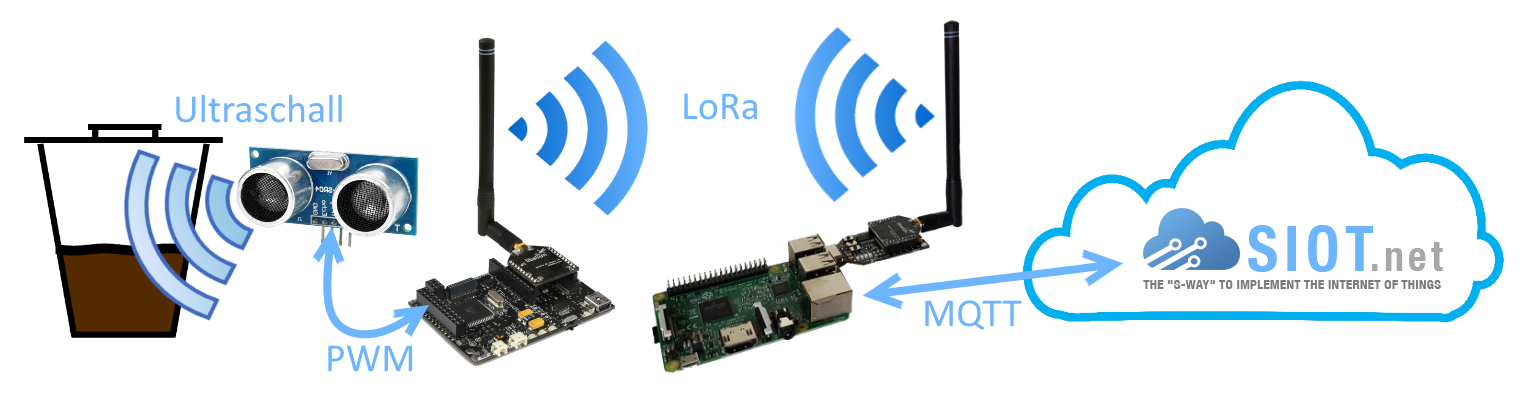
\includegraphics[width=1.0\textwidth]{pictures/PrototypeConcept.png}
    \caption{Gesamt-Architektur des Prototyps inklusive Schnittstellen}
    \label{fig:PrototypeConcept}
\end{figure}

Die Entwicklung des Prototyps bestand aus drei Teilen. Der Erste Teil war die Evaluation von geeigneter Hardware für den \gls{iotk} und den \gls{iotg}. Als nächstes musste die Hardware zusammengebaut werden, wobei hier ein massgeschneidertes Gehäuse modelliert und per 3D-Druck produziert wurde. Parallel zur Entwicklung der Hardware wurde die Software für den Raspberry Pi und den Waspmote entwickelt. 

\section{Hardware}

\subsection{\gls{iotk}-Evaluation}
Für die Evaluation des Knoten wurden verschiedene Embedded-Plattformen in Betracht gezogen. Da dies noch vor der definitiven Entscheidung für \gls{lora} geschah, sind bei den Plattformen auch andere Funktechnologien berücksichtigt worden.

\subsubsection*{Sming}
Sming basiert auf dem TWX51-Sensorknoten, welcher von Daniel Meer an der BFH/TI entwickelt wurde. Herr Meer beschreibt den TWX51 wie folgt: 
\begin{quote}
\textit{Der TXW51 ist ein kleiner und energiesparender Sensorknoten, der als Basis für zukünftige Projekte verwendet werden
kann. Er kommuniziert über Bluetooth Smart und enthält einen Sensor zur Messung der Beschleunigung. Die Firmware kann einfach für neue Anforderungen modifiziert werden.}\autocite{bfh:TXW51}
\end{quote}

\begin{figure}[H]
     \centering
        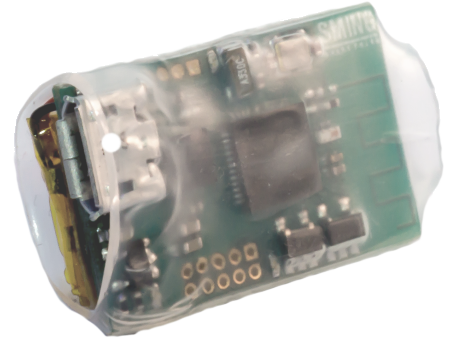
\includegraphics[scale=0.6]{pictures/Sming.png}
    \caption{Sming mit Akku bestückt}
    \label{fig:Sming}
\end{figure}

\textbf{Vorteile}
\begin{itemize}
\item Eigenentwicklung der BFH/TI, komplett internes Wissen
\item Optimiert für tiefen Energieverbrauch
\item sehr kleine Grösse (2.5cm x 1.7cm)
\item hat eine integrierte \gls{ble}-Schnittstelle
\end{itemize}
\textbf{Nachteile}
\begin{itemize}
\item kann zwar über Interrupts aufgeweckt werde, hat jedoch keine RTC
\item hat nur 3V-Spannung (nicht 3.3V), dadurch inkompatibel zu 5V-Sensoren
\item nur kurze Reichweite aufgrund von BLE
\item keine Langdistanz Funktechnik
\end{itemize}

\newpage

\subsubsection*{TinyMesh}
TinyMesh ist das Produkt des gleichnamigen Unternehmens aus Norwegen. Die Idee hinter diesem Produkt ist ein sich selbstformendes und selbstheilendes Sensor-Mesh-Netzwerk zu konstruieren, welches die Sensordaten der einzelnen Knoten an eine Cloud anbindet. Die Knoten basieren auf Modulen von Radiocraft, welche den proprietären TinyMesh-Protokollstack implementieren. Für die Evaluation erhielten wir ein Starter-Kit zum Testen.

\begin{figure}[H]
     \centering
        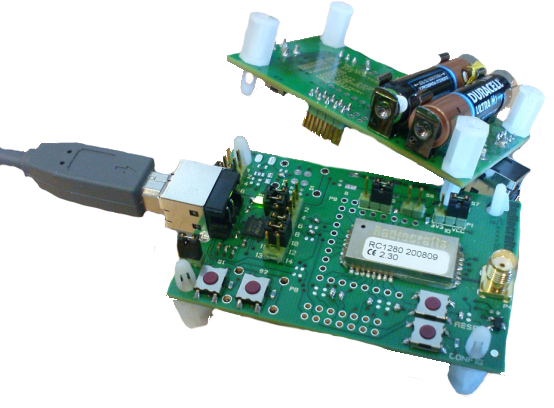
\includegraphics[scale=0.5]{pictures/TinyMesh.png}
    \caption{Radiocraft-Modul und die Batteriehalterung auf der Unterseite}
    \label{fig:TinyMesh}
\end{figure}

\textbf{Vorteile}
\begin{itemize}
\item Mesh-Netzwerk ermöglicht Erweiterung durch Knoten
\item Mesh-Netzwerk ist selbstheilend
\item Mesh-Netzwerk ist selbstkonfigurierend
\end{itemize}
\textbf{Nachteile}
\begin{itemize}
\item Proprietärer TinyMesh Protokollstack
\item Module sind nicht programmierbar, Logik muss von externem Plattform implementiert werden
\item hoher Energieverbrauch durch Mesh-Topologie
\end{itemize}

\newpage

\subsubsection*{Waspmote}
Waspmote\footnote{Waspmote: \url{http://www.libelium.com/products/waspmote/hardware/}} ist eine Mikrocontroller-Plattform der spanischen Firma \gls{libelium}. Die Plattform ist Modular aufgebaut und unterstützt verschiedenste Funktechniken wie \gls{zigbee}, 3G/GPRS und unter anderem auch \gls{lora}. Durch das modulare Design können Funkchips schnell ausgewechselt werden. Die Plattform ist praktisch um Prototypen zu erstellen, wird von \gls{libelium} aber auch als Produkt in Kombination mit über 100 verschiedenen Sensoren vertrieben.
\begin{figure}[H]
     \centering
        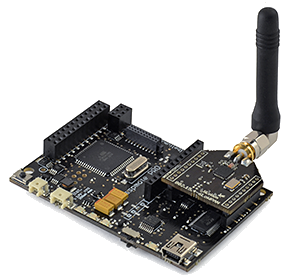
\includegraphics[scale=1.0]{pictures/Waspmote.png}
    \caption{Libelium Waspmote}
    \label{fig:Waspmote}
\end{figure}

\textbf{Vorteile}
\begin{itemize}
\item Modular aufgebaut und ideal für einen Prototyp
\item unterstützt viele Funktechnologien
\item hat eine RTC und kann den Mikrocontroller deaktivieren um den Energieverbrauch zu minimieren. (0.6µA Verbrauch wenn nur RTC in Betrieb)
\item viele GPIOs 
\end{itemize}
\textbf{Nachteile}
\begin{itemize}
\item relativ gross (7.3cm x 5.1cm)
\item teuer (allein ein Waspmote kostet 163 Euro, stand 24.06.2016)
\item verhältnismässig hoher Energieverbrauch im Betrieb (15mA). Die Ursache dafür sind die vielen GPIO's was gleichzeitig auch ein Vorteil ist
\end{itemize}

\subsection*{Entscheidung}
Mit dem Entscheid, ein \gls{lora}-Netzwerk einzusetzen, gehörte Waspmote bereits zu den Favoriten. Das Sming hätte zwar auch mit einem \gls{lora}-Chip verbunden werden können, dies wäre jedoch eher ein Projekt für Studenten der Elektrotechnik. Das Waspmote überzeugt mit seiner Modularität, dem Vorhandensein einer RTC und nicht zuletzt auch damit, dass die Plattform auch schon von Roger Jaggi und Pascal Bohni erfolgreich eingesetzt wurde.

\subsection{Distanz-Sensor}
Wie in Kapitel \ref{chapter:devOfUseCase} beschrieben wird der Füllstand des Mülleimers mittels Ultraschall gemessen. Für diese Distanzmessung wird der Ultraschall-Sensor "HC-SR04" eingesetzt. Er hat einen Messbereich von 2 bis 500cm. Dieser Messbereich beinhaltet alle Distanzen, welche in allen handelsüblichen Mülleimern gemessen werden können. Falls eine Version für Container erstellt werden sollte, müsste ein Sensor mit grösserem Messbereich verwendet werden. 
\begin{figure}[H]
     \centering
        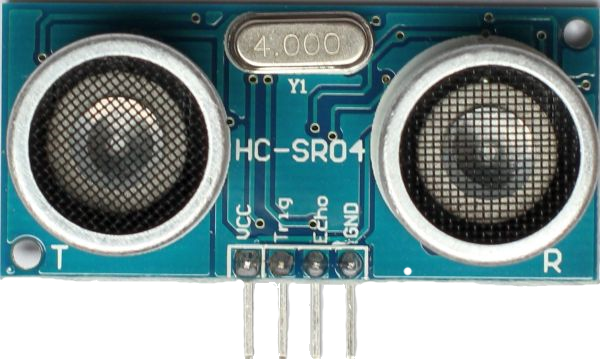
\includegraphics[scale=0.3]{pictures/HC-SR04.png}
    \caption{Ultraschall-Sensor HC-SR04}
    \label{fig:HCSR04}
\end{figure}

\subsection{\gls{iotg}}
Als \gls{iotg} wurde ein Raspberry Pi 3 eingesetzt. Dieser kleine, flexible Einplatinencomputer bietet viele Schnittstellen an, lässt die Wahl zwischen verschiedenen Betriebssystemen und hat eine grosse Community. Für den Anwendungsfall des Tresh-Gateways sind die Netzwerkschnittstellen, um das Gateway mit dem Internet zu verbinden und die USB-Schnittstellen, um das Waspmote Gateway\footnote{Waspmote Gateway: \url{http://www.libelium.com/products/waspmote/interfaces/\#gateway_marker}} an das Raspberry Pi anzuschliessen, essenziell. Das Raspberry Pi 3 bietet dazu zusätzlich zur Ethernet Schnittstelle auch gleich ein fest eingebautes \gls{wlan} Modul an, was viel Flexibilität bei der Platzierung des Gateways ermöglicht. Nichtsdestotrotz ist natürlich die Ethernet-Schnittstelle zu bevorzugen, da diese eine stabilere Netzwerkverbindung zur Verfügung stellt als die \gls{wlan} Schnittstelle. 

\section{Hardware-Implementation}
Nachdem die die Hardware verfügbar war, wurde ein erster Proof-of-Concept aus Holz mit einem grossen Breadboard erstellt. Dieser Prototyp hatte hardwareseitig bereits die volle Funktion. Softwareseitig konnte er ganz rudimentär die gemessene Distanz via \gls{lora} versenden.

\begin{figure}[H]
     \centering
        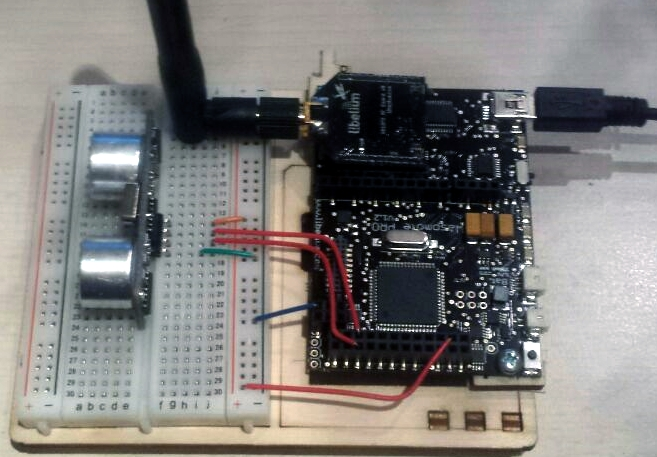
\includegraphics[scale=0.6]{pictures/Prototype1.jpg}
    \caption{Erster Prototyp des \gls{iotk}}
    \label{fig:HCSR04}
\end{figure}

Damit dieser Knoten jedoch in einem Mülleimer eingebaut werden kann, braucht er ein schützendes Gehäuse, damit er einerseits nicht einfach verschmutzt und andererseits stabil im Eimer montiert werden kann. Mithilfe der Open Source Software OpenSCAD konstruierten wir ein zweistöckiges Gehäuse. Im oberen Teil ist das Waspmote und ein kleines Breadboard für den Ultraschall-Sensor untergebracht, im unteren Stock ist Platz für die Batterie. Die Batterie ist ein 6600mAh-Akkumulator, welcher von Libelium für das Waspmote angeboten wird. 
 
\begin{figure}[H]
     \centering
        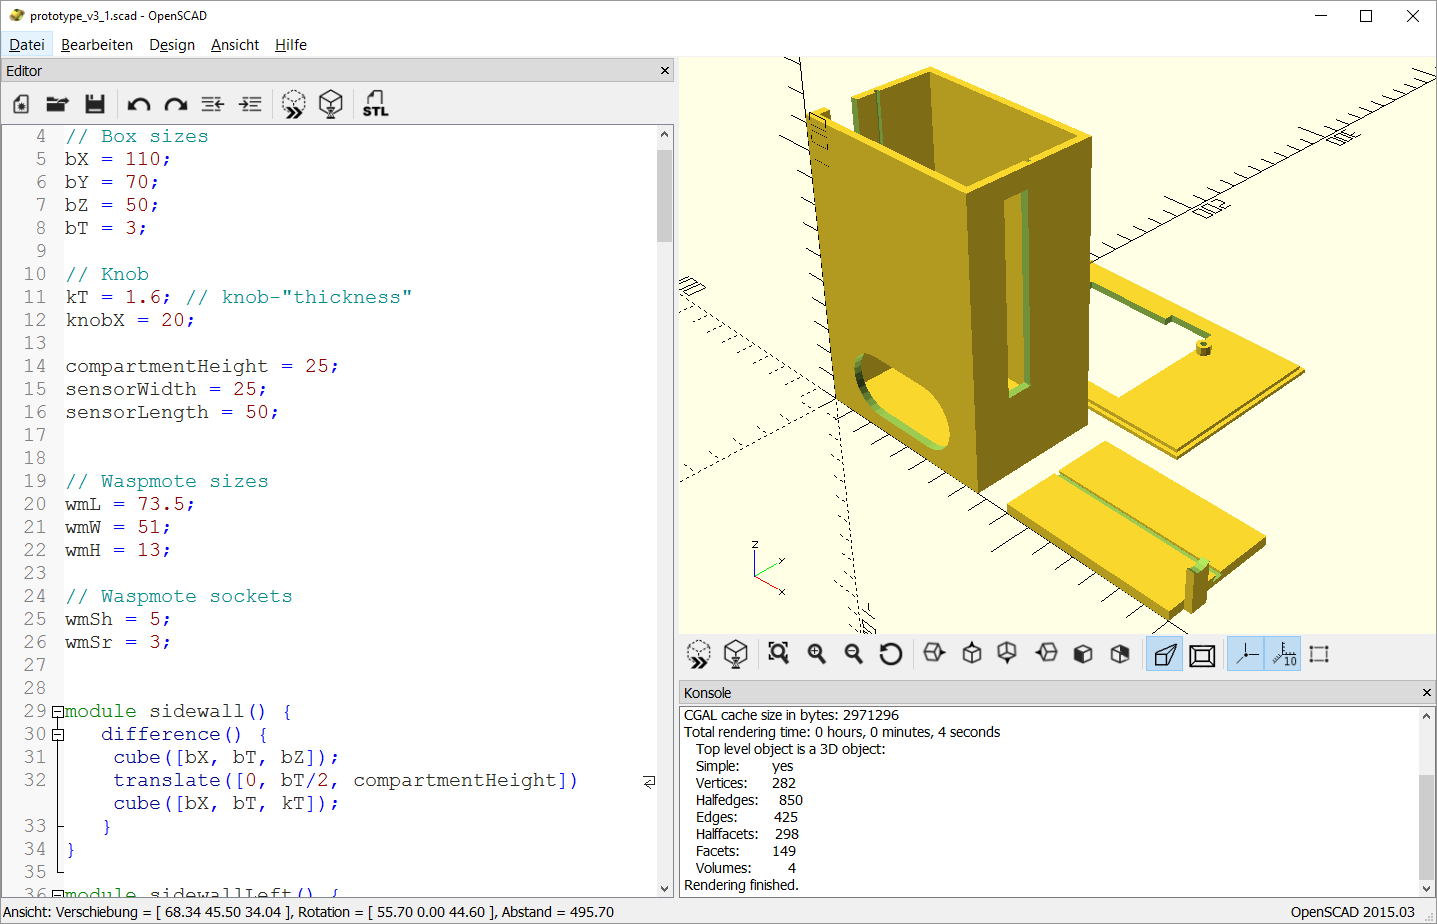
\includegraphics[width=1.0\textwidth]{pictures/OpenSCAD.png}
    \caption{Entwicklung des Gehäuses für den Prototyp}
    \label{fig:OpenSCAD}
\end{figure}

Das Konzept des Gehäuses ist ein Schubladensystem. Das bedeutet, dass die Platine, welche die beiden Kammern des Gehäuses trennt, wie ein Schlitten in das Gehäuse einfahrbar ist. Auf dieser Platte wir auch das Waspmote und der Sensor montiert. Dies hat den Vorteil, dass bei einem Wartungszugriff die ganze Hardware einfach aus dem Gehäuse gezogen werden kann.
Das Gehäuse druckten wir auf einem 3D-Drucker der Firma Ultimaker aus. Es benötigte mehrere Testdrucks und verschiedenste Anpassungen am Plan, bis das Gehäuse mit allen Komponenten zusammenpasste. Besonders delikat war das Schubladensystem, da der Schlitten mit 1mm Dicke nur gerade das zehnfache der Genauigkeit des 3D-Druckers ist.

\begin{figure}[H]
     \centering
        \includegraphics[width=0.55\textwidth]{pictures/3D-Print.jpg}
    \caption{Druck eines Gehäuse-Prototyps mit Ultimaker}
    \label{fig:3D-Print}
\end{figure}

Nachdem alle Gehäusekomponenten zusammenpassten und das Waspmote und das Breadboard montiert werden konnten, starteten wir die erste kleine Serienproduktion von drei kompletten Prototyp \glspl{iotk}.

\begin{figure}[H]
     \centering
        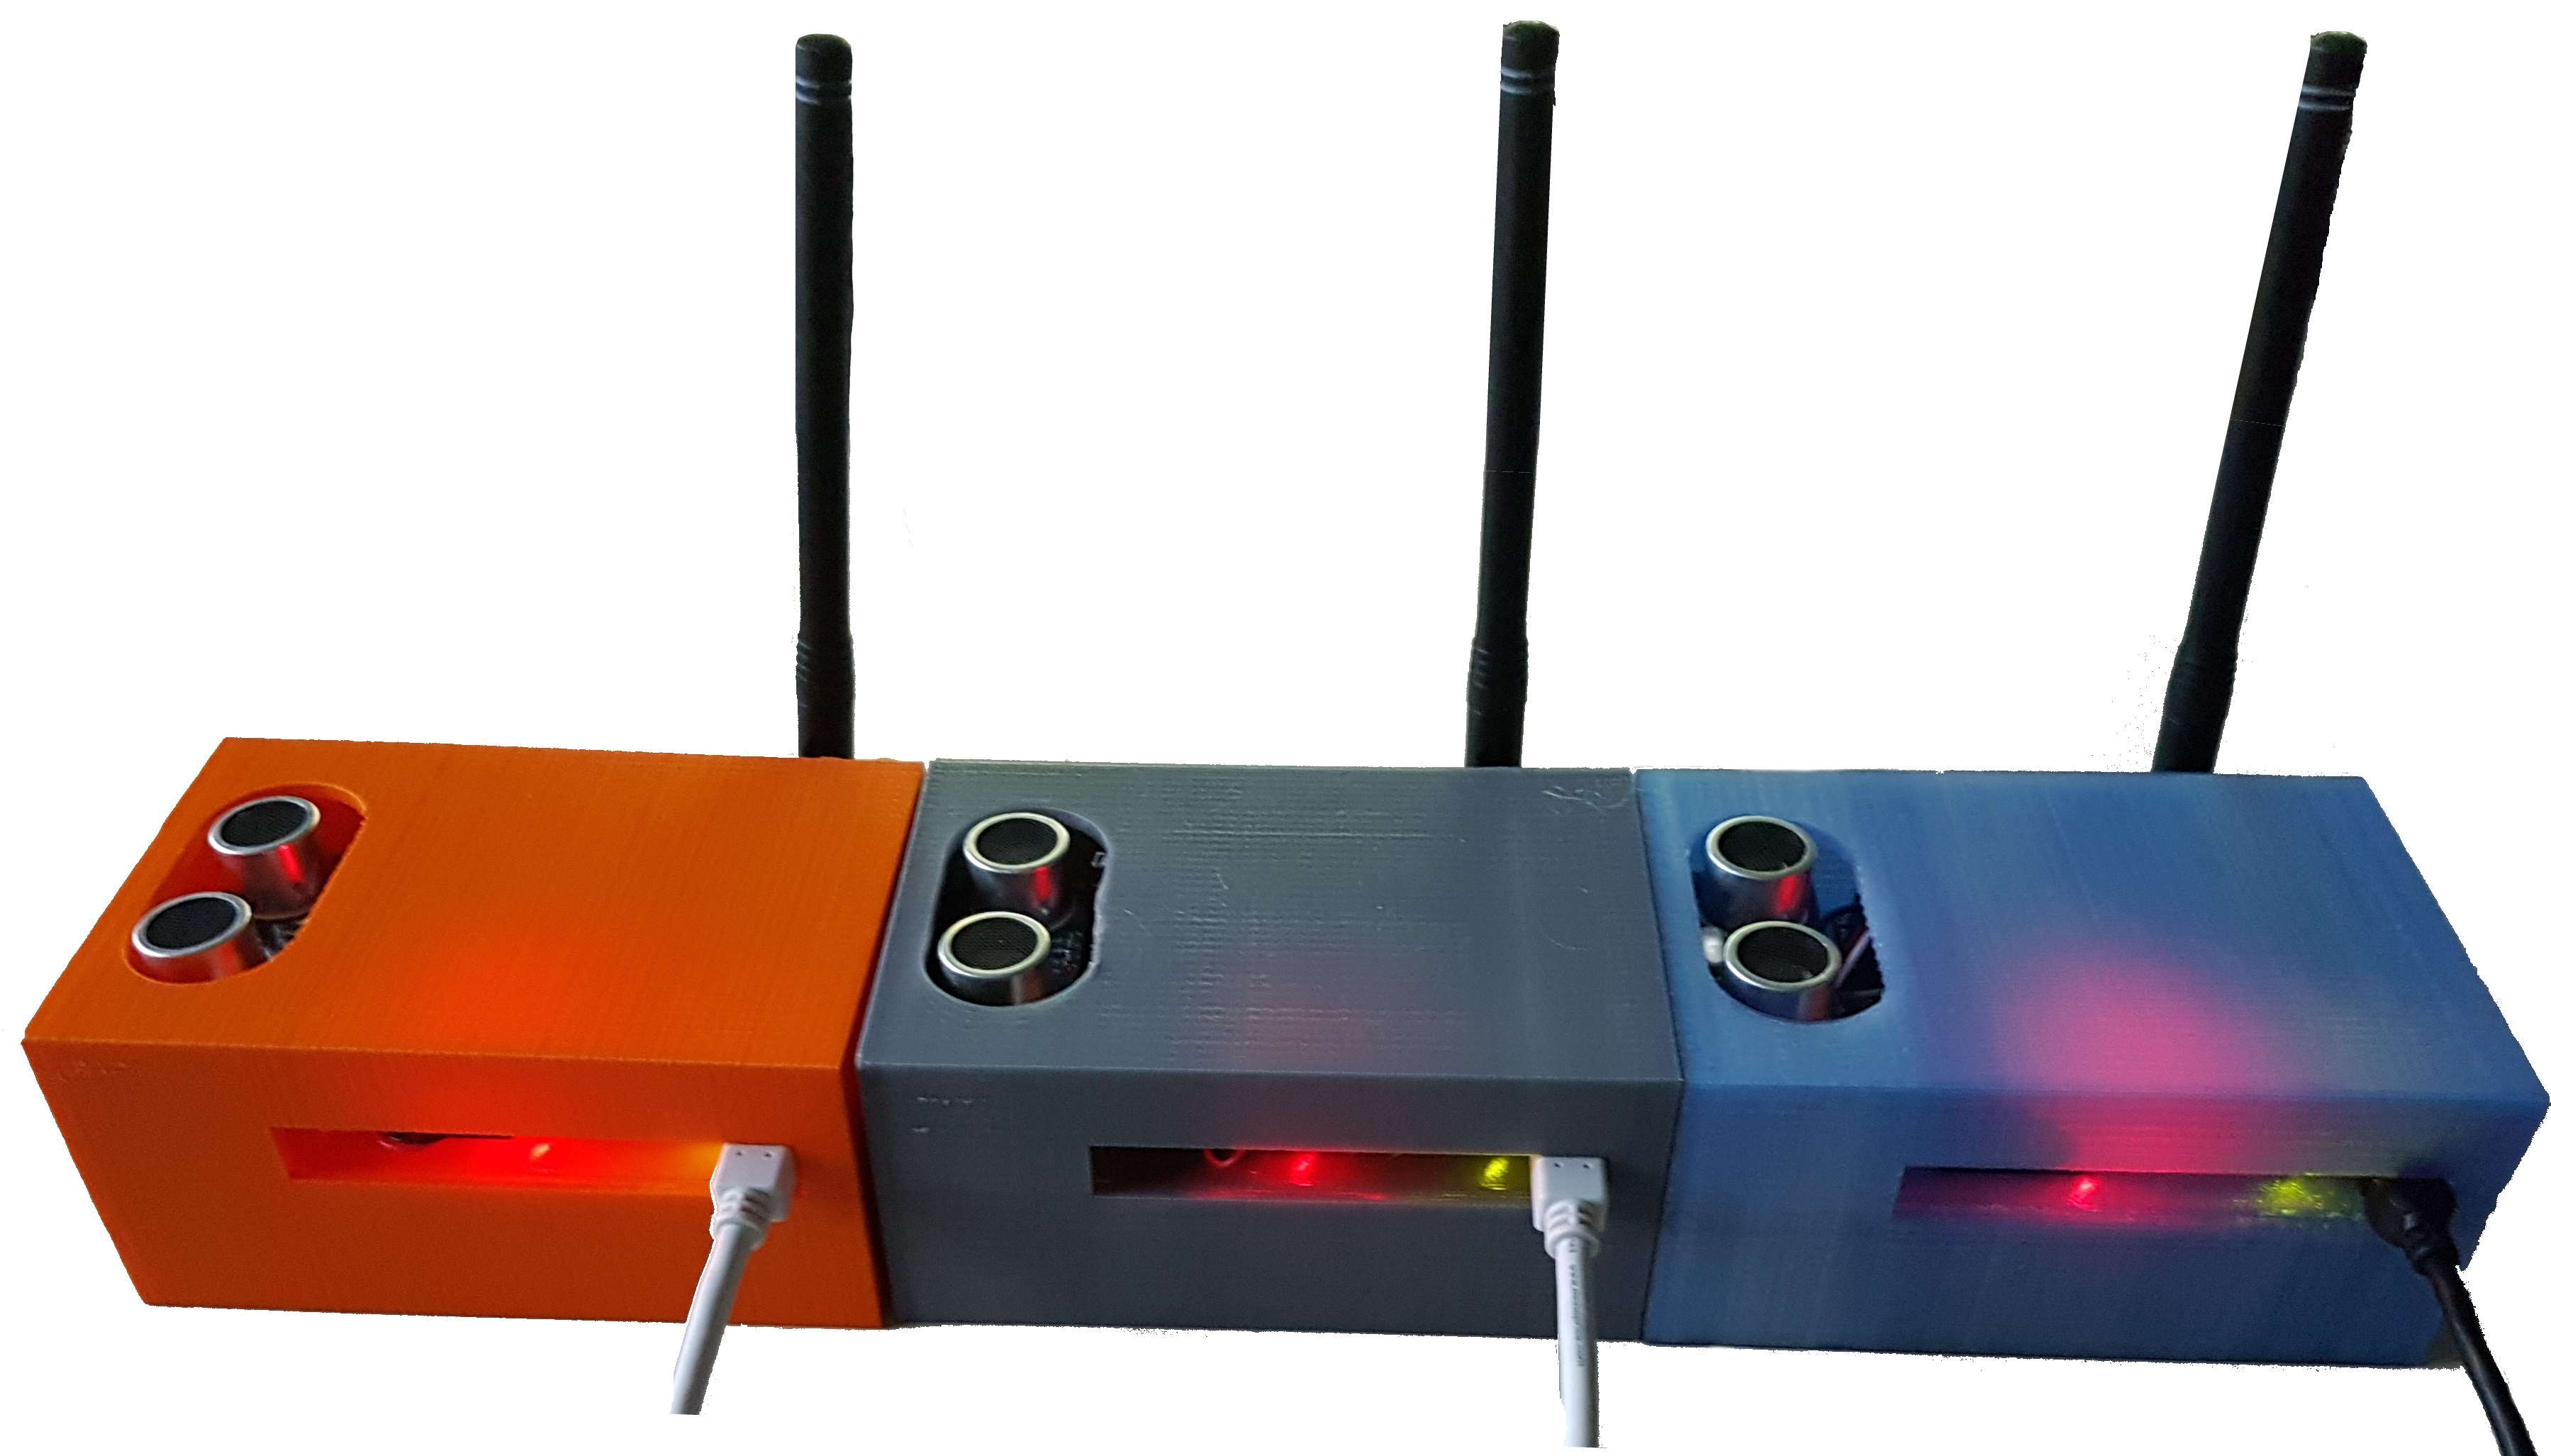
\includegraphics[width=0.8\textwidth]{pictures/Massproduction.jpg}
    \caption{Die drei fertigen Prototypen mit angeschlossenen Ladekabeln}
    \label{fig:3-Prototypes}
\end{figure}

Als nächstes mussten die Prototypen natürlich auch in den Einsatz gebracht werden. Als Testumfeld wurden zusammen mit Herr Danuser die PET-Eimer des Rolex-Gebäudes der BFH in Biel ausgewählt. Herr Danuser holte bei Herrn Schüpbach, dem Leiter des Hausdienstes, die Erlaubnis ein. Dieser erlaubte uns, im PET-Eimer in der Mensa und im PET-Eimer im 5. Stock des Gebäudes einen Sensor zu platzieren.

\subsection*{Installation}
Zwei Wochen vor Projektende konnten wir die Sensoren an ihren Standorten platzieren. Für den Raspberry Pi mit dem Waspmote-Gateway stellte uns Herr Danuser sein Büro zur Verfügung, damit dieser eine konstante Energiequelle sowie Ethernet-Anschluss hat.
Dabei mussten wir feststellen, dass die Frequenzspreizungsmodulation von \gls{lora} definitiv nötig ist, damit das Gateway die Daten des Sensors in der Mensa noch empfängt. Der Sensor sendet mit 7dBm Ausgangsleistung, das Gateway hat mit dem maximalen Spreizfaktor von \gls{lora} eine Empfindlichkeit von -136dBm. Dies ergibt ein Powerbudget von 143dBm, welches auch ziemlich ausgereizt wird. Das Gateway sendet jeweils eine Ack-Bestätigung, wenn ein Sensor ein Paket versandt hat. Damit diese Ack-Pakete garantiert ankommen, sendet das Gateway mit 14dBm.

\begin{figure}[H]
     \centering
        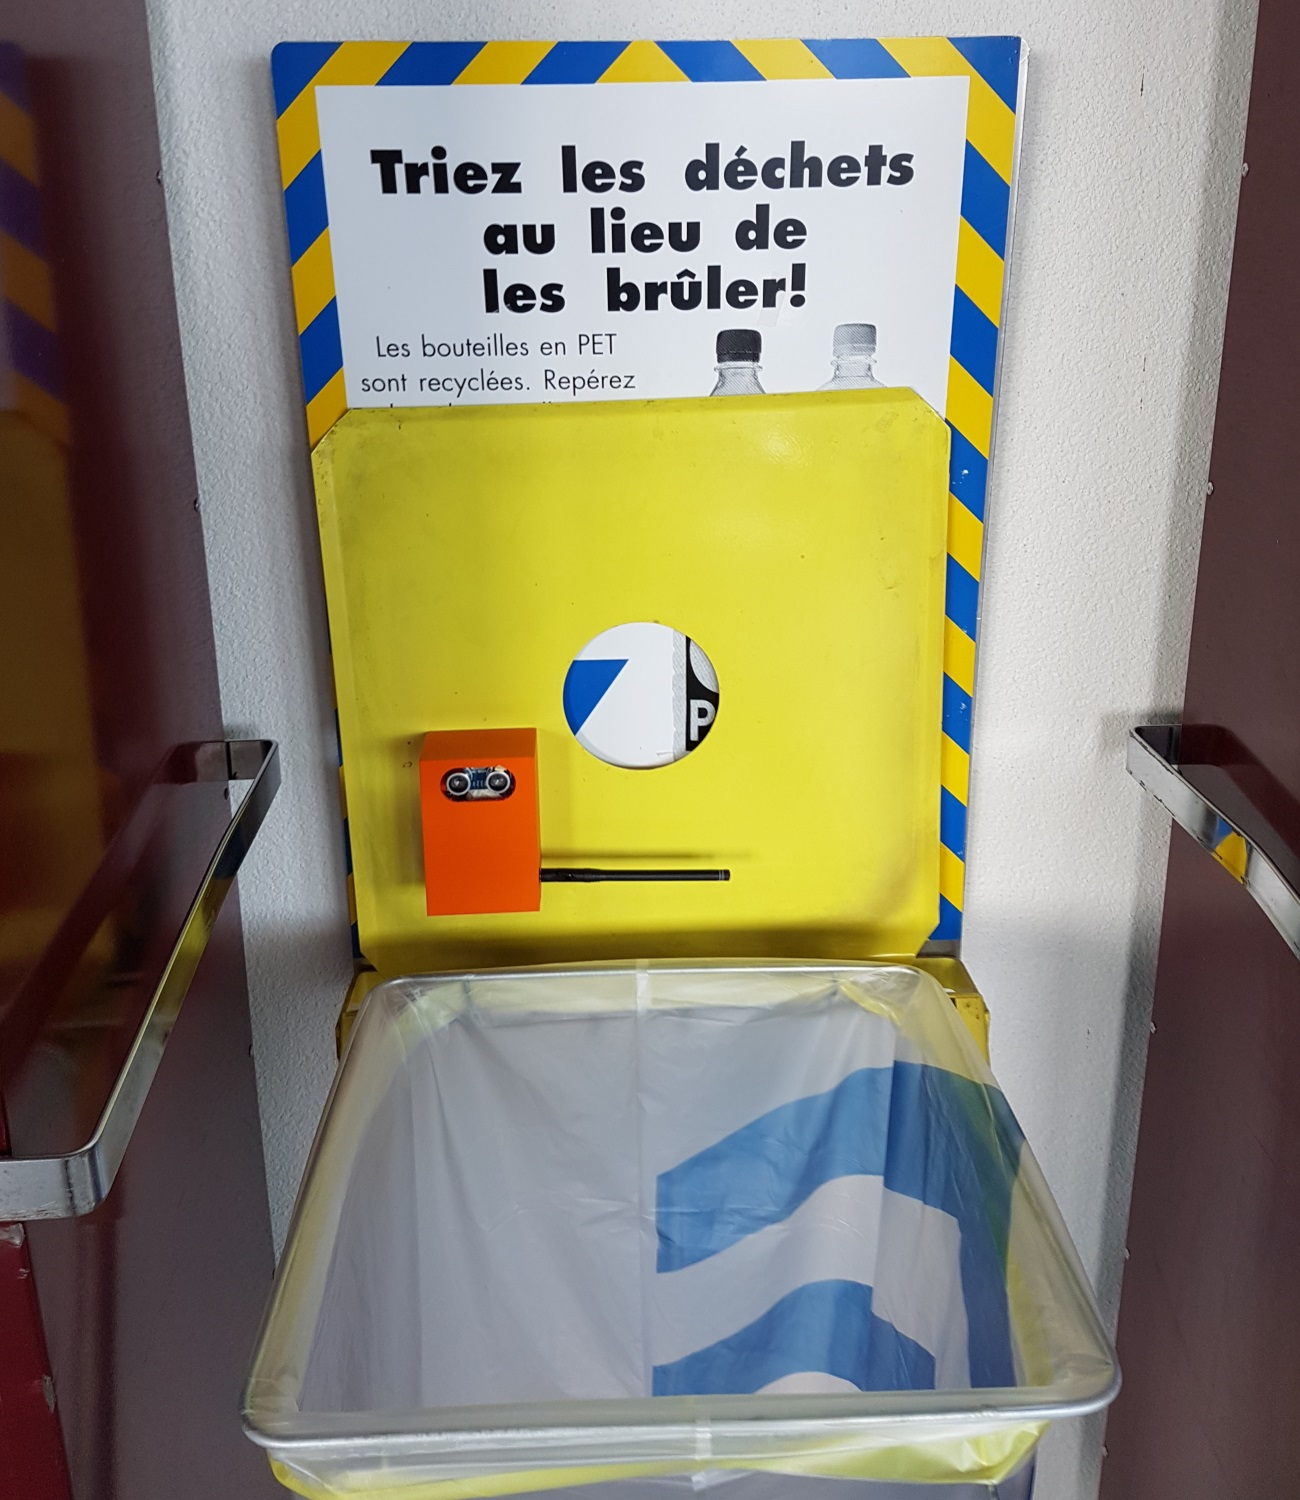
\includegraphics[width=0.7\textwidth]{pictures/Tresh-Deployed.jpg}
    \caption{Der am aufgeklappten Deckel des PET-Eimers in der Mensa befestigte Prototyp}
    \label{fig:3-Prototypes}
\end{figure}

Der zweite Sensor im 5. Stock konnte leider nicht installiert werden. Der dortige Eimer ist komplett aus Metall konstruiert. Sobald der Sensor im Eimer eingeschlossen ist, wird sein Signal durch Reflexionen und Dämpfung des Eimers um ungefähr 45dBm gedämpft. Das restliche Powerbudget von 98dBm reicht leider nicht aus um das Gateway in Herrn Danusers Büro zu erreichen. Der Prototyp bräuchte ein Koaxialkabel, damit seine Antenne ausserhalb des Eimers befestigt werden könnte und nur über das Koaxialkabel mit dem Prototypen im Eimer verbunden wäre.


\section{Software}

\subsection{Waspmote als \gls{iotk}}
Der Waspmote wird mithilfe der Waspmote-IDE programmiert. Diese IDE ist ein Fork der Arduino-IDE und somit für Arduino-Programmierer problemlos zu bedienen.
Die Hauptaufgabe des Waspmote \gls{iotk} ist es, die Distanz zu messen und anschliessend via \gls{lora} an das Gateway zu senden. Der Quellcode ist im Anhang unter \ref{appendix:waspmote} zu finden. Nachfolgend eine Erläuterung dazu.

\textbf{Messung} \\
Da ein Sensor nicht immer zuverlässige Daten liefert, wenden wir für das Auslesen einen kleinen Algorithmus an: Zuerst werden 10 Messungen der Distanz durchgeführt. Danach wird von den 10 Messungen der grösste und der kleinste Wert gesucht. Anschliessend wird ausgewertet, wie oft der minimale und wie oft der maximale Wert gemessen wurde. Je nachdem, wie oft diese Werte vorkommen, wird danach der Durchschnitt der restlichen Werte zurückgegeben, oder aber das Minimum oder das Maximum, abhängig davon welcher mehr vorkam. Damit wird verhindert, dass ein einzelner Ausreisser die Messung verfälscht, gleichzeitig aber auch ein korrekter Wert erscheint, wenn alle Messungen so nahe beieinander sind, dass alle ein Maximum oder ein Minimum bilden.
Zusätzlich werden noch der Batterieladestand und die Temperatur des RTC ausgelesen. Da diese drei Werte alles 16bit integers sind, müssen diese in je zwei 8bit Integer umgewandelt werden, da das \gls{lora}-Modul nur 8bit-Integer versenden kann.

\textbf{Übertragung} \\
Die drei Werte werden anschliessend dem \gls{lora}-Modul als Byte-Array übergeben. Dieses wird erst jetzt hochgefahren, um möglichst wenig Energie zu verbrauchen. Sobald das Modul das Paket versendet hat und ein Ack erhalten hat, wird es wieder heruntergefahren, und der gesamte Mikrocontroller wird für eine Minute deaktiviert, bis der RTC wieder einen Interrupt auslöst. Falls das Modul kein Ack erhält, wartet es eine zufällige Zeit zwischen 1 und 20 Sekunden und versucht es nochmals. Falls dies wieder fehlschlägt, gibt es auf und schaltet sich aus, wie wenn das Ack angekommen wäre.
Die Zeit von 1-20 Sekunden haben wir nach mehreren Kollisions-Tests evaluiert. Auf dem maximalen Spreizfaktor von \gls{lora} können vom Versand des Pakets bis zum Erhalt des Acks 10 Sekunden verstreichen.


\subsection{Raspberry Pi als \gls{iotg}}

Die Hauptfunktion eines \gls{iotg} ist es ein Sensornetzwerk mit einer \gls{iotp} zu verbinden. Genau diese Funktion wurde auf dem Raspberry Pi durch zwei Softwarekomponenten implementiert:

\begin{enumerate}
	\item tresh-lora-gateway - Sensordaten aus dem \gls{lora}-Netzwerk auf dem Waspmote Gateway empfangen.
    \item tresh-siot-gatway - Sensordaten des Waspmote Gateway an die \gls{siot} \gls{iotp} senden.
\end{enumerate}

Der dazugehörige Quellcode ist im Anhang unter \ref{appendix:raspberrypi} aufgeführt.

\subsubsection*{tresh-lora-gateway}

Diese Softwarekomponente empfängt die \gls{lora}-Pakete und gibt sie über die serielle Schnittstelle aus (an das Raspberry Pi). Vor der Ausgabe konvertiert sie die Daten: Das 6-Byte-Array, welches der Sensor zur Übertragung via \gls{lora} generiert hat, splittet das Gateway auf und generiert wieder drei 16bit-Integers. Danach erstellt es ein JSON-Objekt und fügt die Sensor-Daten, sowie die Quelladresse und die RSSI und SNR des Pakets ein und gibt es schliesslich aus.

\begin{lstlisting}[caption=Struktur des JSON-Objekts,numbers=none]
        {"address": <adresse>, "distance": <distanzwert>, "battery": <batteriewert>,
              "temp": <temperatur>, "SNR": <snrwert>, "RSSI": <rssiwert>}
\end{lstlisting}

\subsubsection*{tresh-siot-gatway}
Die Aufgabe dieser Softwarekomponente ist es die Sensordaten über die serielle Schnittstelle zu empfangen und über \gls{mqtt} an die \gls{siot} \gls{iotp} weiterzuleiten. In der Bachelor Thesis \autocite{bfh:optimizedDataTransmission} hat Roger Jaggi die \gls{nodejs}-Applikation siot.net-nodejs-api\autocite{bfh:siot.net-nodejs-api} geschrieben, welche die \gls{siot} Gateway API Spezifikation implementiert. Die tresh-siot-gatway Applikation baut auf dieser API auf. Wir haben zusätzlich das Auswählen und Auslesen des seriellen Ports und die Zuweisung der empfangenen Sensordaten an die entsprechenden, in \gls{siot} registrierten Sensoren implementiert. Diese Zuweisung geschieht anhand der \gls{lora} Netzwerkadresse der ankommende Pakete. Aktuell ist dies eine auf dem Gateway gespeicherte Zuweisungstabelle. In Zukunft sollte diese Zuweisung aber dynamisch konfigurierbar sein, so dass neue Sensor-Knoten ohne die Rekonfiguration des Gateways hinzugefügt werden können.

\subsection{\gls{siot}}
Nachdem die Sensoren von unserem Gateway im \gls{siot} registriert wurden, sind sie nun im Dashboard verfügbar zur Darstellung. Wir haben ein Dashboard erstellt, welches von sämtlichen Sensoren den aktuellen Wert, sowie einen Graphen der letzten 1000 Werte darstellt. Eine Woche nachdem wir die \gls{iotk} in Betrieb nahmen, wurde von \gls{siot} ein neuer Release veröffentlicht. Dieser bewirkte, dass alle unsere Graphen nicht mehr dargestellt wurden. In Abklärung mit den Entwicklern von \gls{siot} erfuhren wir, dass neu jeder Sensor, dessen Daten auch gespeichert werden sollen, nun im Manifest-JSON den Eintrag \verb|"storage":"db"| haben muss, damit die Werte überhaupt erst persistiert werden.

\begin{figure}[H]
     \centering
        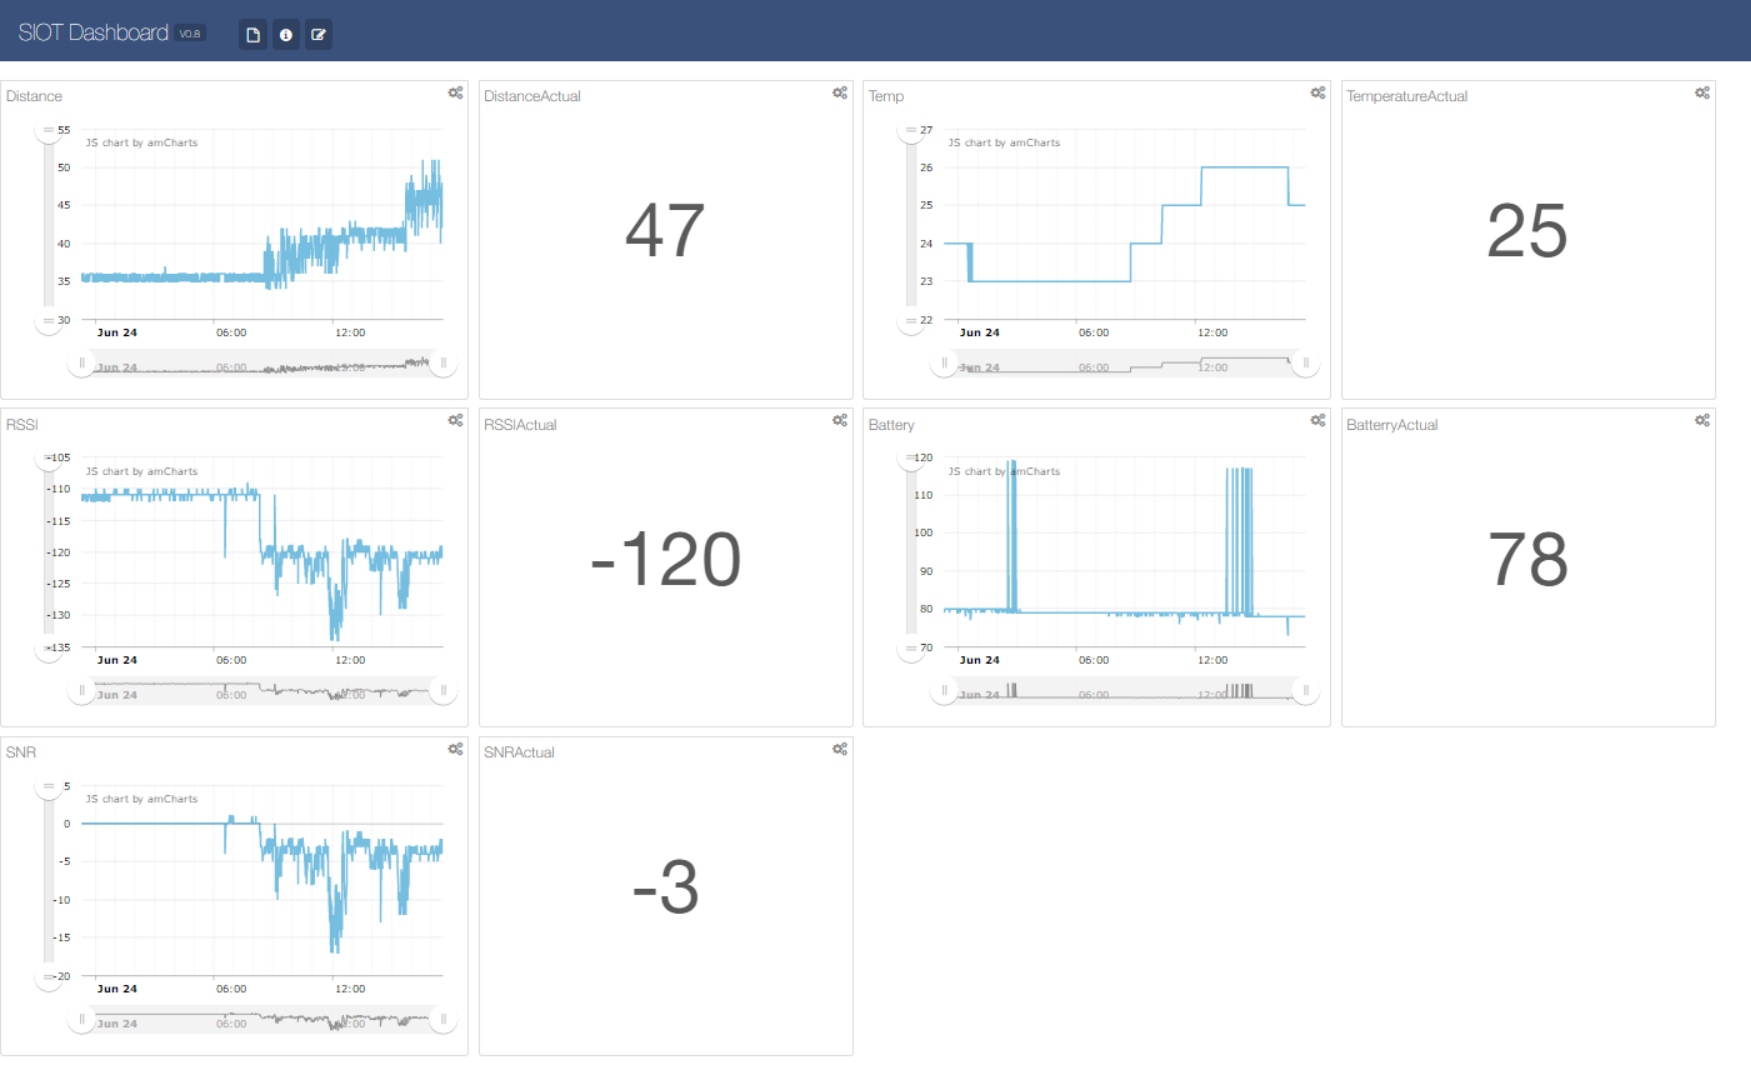
\includegraphics[width=0.9\textwidth]{pictures/SIOT.png}
    \caption{SIOT Dashboard des Prototyps}
    \label{fig:SIOT-Dashboard}
\end{figure}


\section{Resultate}
\subsection*{Füllstand}
Der Füllstand, welcher in Form der Distanz in Zentimetern vom Deckel zum aktuellen Füllstand ausgelesen wurde, liefert zuverlässige Messresultate. 
Trotz der schon im \gls{iotk} integrierten Statistik-Funktionen, sind die Daten immer noch schwankend. Die Schwankungen sind jedoch in einem Bereich von +-5 Zentimetern, was durch die unebenen PET-Flaschen erklärt werden kann.
Mithilfe des von Pacsal Bohni und Roger Jaggi entwickelten Aggregators könnten natürlich noch spezifischere Füllstände berechnet werden. Zum Beispiel indem von der Höhe des Eimers (in unserem Fall 73cm) die gemessene Distanz subtrahiert wird. Auch könnte damit weitere Statistik betrieben werden, beispielsweise indem der Durchschnitt von 3 Messungen genommen wird etc.
Anbei eine Auswertung der Daten über eine Woche. Wir haben versucht die Resultate zu interpretieren und dazu eine kleine Legende gemacht.

\begin{figure}[H]
     \centering
        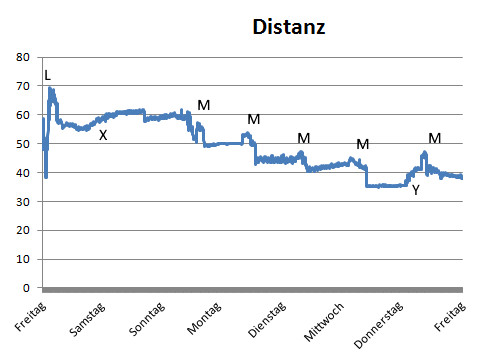
\includegraphics[width=0.9\textwidth]{pictures/Distance-Statistics.png}
    \caption{Füllstand-Distanz über eine Woche}
    \label{fig:Distance-Statistics}
\end{figure}

\textbf{Legende:}
\begin{table}[H]
\begin{tabulary}{\paperwidth}{m{0.08cm} m{15cm}}
L & Leerung: Kurz nach der Installation des Sensors wurde Der Eimer geleert. \\ \hline
M & Mittagessen: Das Mittagessen ist der Event, wo am meisten PET-Flaschen weggeworfen werden. Interessant ist, dass jeweils bevor der Eimer voller wird, jeweils zuerst nochmals mehr Distanz verfügbar ist. Wahrscheinlich lässt sich dies damit erklären, dass durch das Einwerfen der Flaschen, die schon vorhanden Flaschen besser geordnet werden und damit wieder etwas mehr Platz frei wird. \\ \hline
X & Der Eimer leert sich über die Zeit? Mögliche Erklärung: die Flaschen \glqq{}ordnen\grqq{} sich langsam im Eimer während keine neuen eingeworfen werden (da am Samstag kaum Betrieb ist) \\ \hline
Y & Wieder ein \glqq{}Selbstentleerung-Phänomen\grqq{}. Möglicherweise eine extreme Form des Mittagessen-Phänomens?
\end{tabulary}
\end{table}

\subsection*{Batterie}
Die Batterie hat über eine Woche Betrieb 15\% Ladung verloren. Das heisst also, pro Woche verbraucht der Sensor rund 990mA. Mit dem 6600mAh-Akku kann der Sensor also rund 45 Tage durchhalten.
Natürlich gibt es bei unserem Messverhalten noch eine Menge Optimierungspotential. Der Knoten misst und sendet aktuell jede Minute den neuen Füllstand. Dies ist für den Use-Case eigentlich viel zu oft. Wir haben dieses Intervall bestimmt um eine Art \glqq{}Stress-Test\grqq{} unseres Systems zu machen und möglichst rasch an Daten zu kommen. Im echten Einsatz würde es aber reichen, die Messung und Übertragung in grösseren Intervallen durchzuführen. Beispielsweise alle 15 Minuten oder stündlich. Weiter sollte das Messintervall dynamisch der Situation angepasst werden können. Zu Zeiten ohne Betrieb, kann das Intervall viel grösser sein, als bei Betrieb. In unserem Fall könnte also in der Nacht und übers Wochenende ein Intervall von beispielsweise drei oder sechs Stunden gewählt werden. Während den Semesterferien könnte sogar ein Tag als Intervall gewählt werden.
Wenn schon nur das Intervall generell auf eine Stunde gesetzt wird, könnte der Sensor hochgerechnet über 7 Jahre mit einer Akkuladung durchlaufen.
